What follows is a series of queries for particular kinds of questions of interest for CP2K 
application users as well as within  Oak Ridge Leadership Class Facility \acs{OLCF}.
This case study is intended to show how the tool can be used to query an application and to 
demonstrate the level of detail of the queries that can  be of general interest to any \acs{HPC} 
applications.

Queries such as these can be easily compose to work on different fields/attributes, combined, or 
broken apart in any number of ways to manipulate the content of the AST, as well as made with or 
without the use of the dynamic sampling frequencies obtained from user profiling to narrow the 
search space based on the application hotspots.
It is worth noting that for added simplicity, we omit the parts of the queries that filter based upon 
build, application, or profiling IDs as these are unnecessary to understand the queries.

\subsection{CP2K}
\label{sec:cp2k}
CP2K \cite{hutter2014cp2k} is a popular molecular simulation package, written in Fortran 95, that includes numerous routines for quantum chemistry and solid-state physics, including \ac{AIMD} \cite{marx2009ab}.
Molecular dynamics within the \ac{BO} regime simulates atomic motion according to classical mechanics, while forces may be calculated using any type of physics.
For \ac{AIMD}, the forces are calculated using quantum mechanics, via derivatives of the system's electronic potential energy surface.
This energy is usually obtained with a \ac{SCF} calculation with \ac{DFT} \cite{vandevondele2012linear,hutter2014cp2k}, which involves an iterative solver that must converge before the energy is known, and tensor contractions of large tensors representing electron orbitals.
Therefore, each time-step requires considerably more computational time and memory than classical molecular dynamics.
However, \ac{AIMD} is able to explore essential chemical properties such as time-dependent changes in polarization, charge densities, protonation states, and bond breaking and formation, all of which are inaccessible to classical molecular dynamics and of great interest to physicists, chemists and molecular biologists.

Until recently, \ac{AIMD} simulations on systems with thousands of atoms for timescales longer than a few picoseconds was not possible.
Currently, several parallel implementations of the \ac{DFT} based \ac{SCF} calculation have exploited massive parallelization on \acs{HPC} systems to obtain the \ac{SCF} based electronic energy of such large systems in under a minute \cite{vasp_bench,kresse1996efficient,cp2k_bench,vandevondele2012linear}.
This opens up the possibility of simulating, for the first time, electronic-structure-dependent properties as time series extending to hundreds of picoseconds of simulation time, which can be compared to experimental results \cite{gillan2016perspective, pestana2017ab, hassanali2013proton, milovanovic2018new, sellner2013charge}.

The \ac{LS-SCF} calculation \cite{vandevondele2012linear} in CP2K has made use of an algorithm that exploits physical locality to decompose the \ac{SCF} calculation into what effectively becomes sparse matrix multiplication, which is then approached with their own auto-tuning small matrix multiplication library, \texttt{libsmm} \cite{borvstnik2014sparse}.
An Intel-optimized version of this library, \texttt{libxsmm}, has also been created for CP2K by programmers working for Intel \cite{heinecke2016libxsmm}.
In addition, a \acs{GPU} based version is available, and the procedures are all incorporated into the \ac{DBCSR} library \cite{borvstnik2014sparse,schutt2016gpu}, which is the engine for the \ac{LS-SCF} calculation.
Despite these efforts and other extensive optimizations including excellent \acs{MPI} based decomposition, OpenMP threading, and use of parallel libraries such as ScaLAPACK and threaded \ac{FFTW}, CP2K cannot scale to much more than a thousand nodes on supercomputers, resulting in a lack of ability to utilize over 5\% of systems such as the \acs{OLCF}'s Titan, while capability level programs often are able to use much more.
It is programs such as CP2K, therefore, which provide state of the art tools for obtaining cutting edge scientific results, that can benefit greatly from performance analysis tools beyond profilers, in order to potentially further increase their ability to make efficient use of leadership computing resources.


%TODO: NOTES: missing id hacks and omission of ids in listings, interprocedural analysis 
%discussion, library file/module discussion, ...?
\subsection{Finding OpenMP Regions of Interest}
Identifying important the important code regions to port to a new architecture is of extreme important  
for performance and to develop a porting plan to a new architecture.
This query incorporates static and some dynamic profiling 
data to determine where we might want to focus our analysis and/or porting efforts.
We address this problem in two separate steps - determining the characteristics with which we will 
select regions of interest, and finding the set of functions observed in our sampling data with which 
we will restrict our search.
The second part requires enough to merit its own query here, which can be seen in 
Listing~\ref{lst:restrict}.
In this query, we start by selecting all the sampled stack information from our profiler output, located 
in a table called \texttt{stack\_line\_frequency}.
We then proceed to ``unnest'' these stacks to get a series of individual file and line tuples, and match 
the resulting file names to those stored in the database so as to filter out any that weren't included in 
the original export of data (necessary since source level information is not necessarily available for 
all functions that may be in the stack, e.g. for external libraries).
Once we have this, we compare them against any code lines that contain matching line numbers and 
get the names for the containing functions.
Finally, we eliminate duplicates so that we have a distinct set of all functions sampled.

\begin{lstlisting}[caption=Determing Functions Sampled, label=lst:restrict]
select distinct code_lines.ns_proc_name.name
from	(
		select stack_files.file,
		       stack_lines.line
		from	(
				select   files,
				         lines
				from     map.stack_line_frequency
				group by files,
				         lines limit 1) stack
		join   unnest(stack.files) with ordinality as stack_files(file, index)
		on     true
		join   unnest(stack.lines) with ordinality as stack_lines(line, index)
		on     stack_lines.index = stack_files.index
		join	(
				select distinct filename
				from            gcc.gfc_file) file
		on     file.filename = stack_files.file) freq
join	gcc.code_lines as code_lines
on	code_lines.filename = freq.file
and	code_lines.lines @> array[freq.line]
join	gcc.gfc_symbol as sym
on	sym.record_address = code_lines.ns_proc_name
and	sym.build_id = code_lines.build_id;
\end{lstlisting}

Next, we incorporate the previous query into our search as a subquery, which we will simply refer to 
as \texttt{subquery} for simplicity.
This query can be seen in Listing~\ref{lst:omp-search}.
We decided to search among the functions for those that had high numbers of OpenMP parallel regions, under 
the logic that might have the most complex or interesting behavior.
To do this, we search the \texttt{annotated\_code} table for statements that define OpenMP regions 
(i.e., have a reference to a \texttt{gfc\_omp\_clauses} entry in their \texttt{ext.omp\_clauses} field) 
that have an operation type of 75 or 76 (EXEC\_OMP\_PARALLEL and 
EXEC\_OMP\_PARALLEL\_DO, respectively).
Finally, we count the number of such regions for each function and filter for only those that both are 
included in the sampled data and have more than one parallel region, sorting by the number of 
regions counted.
The results of this query can be seen in Table~\ref{tbl:parallel-regions}.

\begin{lstlisting}[caption=Finding High Concentrations of OpenMP Parallel Regions, 
label=lst:omp-search]
select 
sym.name,
       count(sym.name)
from   gcc.annotated_code as annotated
       join gcc.gfc_symbol as sym
         on sym.record_address = annotated.ns_proc_name
            and sym.build_id = annotated.build_id
where  annotated."ext.omp_clauses" is not null
       and annotated.op in ( 75, 76 )
       and sym.name in (select *
                        from   subquery)
group  by sym.name
having count(sym.name) > 1
order  by count(sym.name) desc;  
\end{lstlisting}

\begin{table}[htbp]
\caption{Subroutines with High Numbers of OpenMP Parallel Regions}
\begin{center}
\begin{tabular}{|c|c|c|}
\hline
\textbf{Subroutine} & \textbf{Parallel Regions} \\
\hline
pw\_axpy & 14 \\
\hline
xc\_vxc\_pw\_create & 10 \\
\hline
pw\_copy & 8 \\
\hline
pw\_scatter\_s & 4 \\
\hline
rs\_pw\_transfer & 4 \\
\hline
dbcsr\_data\_copyall & 4 \\
\hline
multiply\_cannon & 4 \\
\hline
pw\_gather\_s & 2 \\
\hline
dbcsr\_multiply\_generic & 2 \\
\hline
build\_core\_ppnl & 2 \\
\hline
\end{tabular}
\label{tbl:parallel-regions}
\end{center}
\end{table}

\subsection{Measuring Variable Use Within OpenMP Parallel Regions}

Finally, we will combine elements of the previous queries to accomplish something truly novel - 
getting a rough measure of performance for each of hundreds of individual variables in OpenMP 
regions based on standard profiler sampling and measuring the effects of varying numbers of 
threads on these measures.
We accomplish this by using the line-based reference counting described in 
Section~\ref{sec:querying}, parts of the previous query to both join the static and dynamic data and 
filter for references occurring within OpenMP regions, as well as the filtering based on function name 
that we first used for finding ScaLAPACK function calls in Table~\ref{tbl:scalapack-funcs}.
Thus, we:
\begin{itemize}
\item Use the output from MAP to get all the sampled stacks from the application and how many 
times they were encountered
\item Match up the file and line numbers to the database to determine which functions those samples 
occurred in
\item Select only the samples that were contained within the top few functions of interest (where we 
observed from profiling that the vast majority of time was spent)
\item Find all variables referenced on those lines and add the sample count from MAP to a running 
total for each variable
\item Group the data together by variable (not lines) and add the counts together for every time each 
variable was accessed across all relevant lines
\item Repeat for the data obtained from multiple runs with different thread counts (1, 2, 4, and 8)
\end{itemize}
The results of this query can be seen in Figure~\ref{fig:openmp-refcount}, where each line 
represents a single variable and the total number of times any thread accessed it across the 
observed samples.
If all parallel regions had a fairly even work distribution across threads and we achieved linear 
speedup, we might expect to see the corresponding lines in the plot be largely flat, representing 
roughly the same total number of accesses but with greater numbers of threads making those 
accesses concurrently.
This also means that what we don't want to see is deviations resulting in increases to the number of 
accesses.
In the plot, we can see that this is the case for a fair number of variables in moving from one to two 
threads, but that access counts for most variables remain fairly constant afterward.
This may be attributable to startup overhead, though the affected variables merit closer investigation.

\begin{figure}
\begin{center}
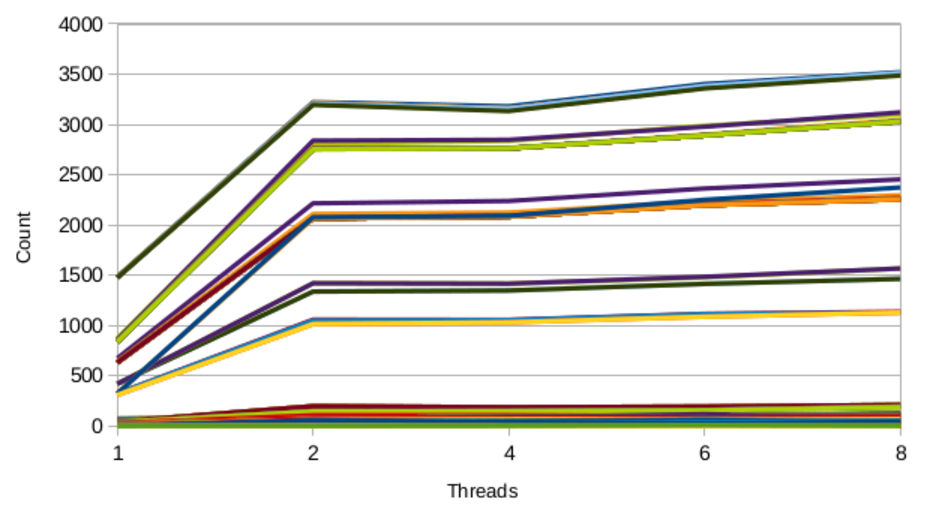
\includegraphics[width=0.45\textwidth]{images/cp2k-omp-inc-full.pdf}
\end{center}
\caption{Sampled Reference Counts to Variables Within OpenMP Parallel Regions}
\label{fig:openmp-refcount}
\end{figure}

\subsection{Determining Use of System and User Libraries}
One of the bigger concerns for \acs{HPC} applications when targeting a new system is determining 
which system resources, 
particularly that of libraries, are actively being used in applications so as to better direct porting 
efforts.
As such, it is valuable to query not just which libraries are linked in (which has already been done by  
tools like XALT), but also the context on which functions within those libraries are actually getting 
called within user code and their call paths.
To this end, we queried CP2K to discover which \ac{FFTW} functions were actually referenced in the 
code.
The query can be seen in Listing~\ref{lst:fftw}, which searches for call statements and joins each one 
with the symbol table on its \texttt{resolved\_sym} field, which is 
used for referencing the called function's symbol, before finally outputting a sorted list of all distinct 
names found for symbols originating from the library module \texttt{fftw3\_lib}.
The results can be seen in Table~\ref{tab:fftw-funcs}.

\begin{lstlisting}[caption=Querying for Use of Library Functions, label=lst:fftw]
select distinct sym.name
from   gcc.gfc_code as code
       join gcc.gfc_symbol as sym
         on sym.record_address = code.resolved_sym
            and sym.build_id = code.build_id
where  code.op = 10
       and sym.module = 'fftw3_lib'
order  by sym.name;
\end{lstlisting}

\begin{table}[htbp]
\caption{FFTW Subroutines Referenced}
\begin{center}
\begin{tabular}{|c|}
\hline
\textbf{Subroutine} \\
\hline
fftw31dm \\
\hline
fftw33d \\
\hline
fftw3\_compute\_rows\_per\_th \\
\hline
fftw3\_create\_3d\_plans \\
\hline
fftw3\_create\_guru\_plan \\
\hline
fftw3\_create\_plan\_1dm \\
\hline
fftw3\_create\_plan\_3d \\
\hline
fftw3\_destroy\_plan \\
\hline
fftw3\_do\_cleanup \\
\hline
fftw3\_do\_init \\
\hline
fftw3\_get\_lengths \\
\hline
fftw3\_workshare\_execute\_dft \\
\hline
fftw\_cleanup \\
\hline
fftw\_export\_wisdom\_to\_file \\
\hline
fftw\_import\_wisdom\_from\_file \\
\hline
sortint \\
\hline
\end{tabular}
\label{tab:fftw-funcs}
\end{center}
\end{table}

The same general form of query could be narrowed down in a couple other ways as well.
In addition to filtering function symbols by module(s), one could also filter based on which file(s) they 
are found in, or module
A user may also want to know more detailed information about invocations, particularly the file/line 
locations each can be found at.
Table~\ref{tbl:scalapack-funcs} shows an example of exactly this, showing the file and line numbers 
found for calls to ScaLAPACK subroutines.
The results have been limited to the top 15 for brevity.

\begin{table}[htbp]
\caption{ScaLAPACK Subroutine Reference Locations}
\begin{center}
\begin{tabular}{|c|c|c|}
\hline
\textbf{File} & \textbf{Lines} & \textbf{Subroutine} \\
\hline
src/cp\_dbcsr\_cholesky.F & {103} & pspotrf \\
\hline
src/cp\_dbcsr\_cholesky.F & {105} & pdpotrf \\
\hline
src/cp\_dbcsr\_cholesky.F & {187} & pspotri \\
\hline
src/cp\_dbcsr\_cholesky.F & {189} & pdpotri \\
\hline
src/fm/cp\_cfm\_basic\_linalg.F & {411} & pzgetrf \\
\hline
src/fm/cp\_cfm\_basic\_linalg.F & {703} & pzgetrf \\
\hline
src/fm/cp\_cfm\_basic\_linalg.F & {736,737} & pzgetrs \\
\hline
src/fm/cp\_cfm\_basic\_linalg.F & {799,800} & pzgetrf \\
\hline
src/fm/cp\_cfm\_basic\_linalg.F & {812,813} & pzgetri \\
\hline
src/fm/cp\_cfm\_basic\_linalg.F & {818,819} & pzgetri \\
\hline
src/fm/cp\_cfm\_basic\_linalg.F & {882} & pzpotrf \\
\hline
src/fm/cp\_cfm\_basic\_linalg.F & {938} & pzpotri \\
\hline
src/fm/cp\_cfm\_basic\_linalg.F & {1147} & pztrtri \\
\hline
src/fm/cp\_cfm\_diag.F & {90,91} & pzheevd \\
\hline
src/fm/cp\_cfm\_diag.F & {121,122} & pzheevd \\
\hline
%src/fm/cp\_fm\_basic\_linalg.F & {300} & pdgetrf \\
%\hline
%src/fm/cp\_fm\_basic\_linalg.F & {1348} & pdgetrf \\
%\hline
%src/fm/cp\_fm\_basic\_linalg.F & {1383} & pdgetrs \\
%\hline
%src/fm/cp\_fm\_basic\_linalg.F & {1400,1401} & pdgesvd \\
%\hline
%src/fm/cp\_fm\_basic\_linalg.F & {1406,1407} & pdgesvd \\
%\hline
%src/fm/cp\_fm\_basic\_linalg.F & {1511} & pdtrtri \\
%\hline
%src/fm/cp\_fm\_basic\_linalg.F & {1576} & pdgeqrf \\
%\hline
%src/fm/cp\_fm\_basic\_linalg.F & {1580} & pdgeqrf \\
%\hline
%src/fm/cp\_fm\_basic\_linalg.F & {1640} & pdgetrf \\
%\hline
%src/fm/cp\_fm\_basic\_linalg.F & {1641,1642} & pdgetrs \\
%\hline
%src/fm/cp\_fm\_basic\_linalg.F & {1776,1777} & psgetrf \\
%\hline
%src/fm/cp\_fm\_basic\_linalg.F & {1779,1780} & pdgetrf \\
%\hline
%src/fm/cp\_fm\_basic\_linalg.F & {1804,1805} & psgetri \\
%\hline
%src/fm/cp\_fm\_basic\_linalg.F & {1810,1811} & pdgetri \\
%\hline
%src/fm/cp\_fm\_basic\_linalg.F & {1820,1821} & psgetri \\
%\hline
%src/fm/cp\_fm\_basic\_linalg.F & {1823,1824} & pdgetri \\
%\hline
%src/fm/cp\_fm\_cholesky.F & {75} & pspotrf \\
%\hline
%src/fm/cp\_fm\_cholesky.F & {77} & pdpotrf \\
%\hline
%src/fm/cp\_fm\_cholesky.F & {143} & pspotri \\
%\hline
%src/fm/cp\_fm\_cholesky.F & {145} & pdpotri \\
%\hline
%src/fm/cp\_fm\_cholesky.F & {211} & pdsygst \\
%\hline
%src/fm/cp\_fm\_diag.F & {359,360} & pdsyevd \\
%\hline
%src/fm/cp\_fm\_diag.F & {380,381} & pdsyevd \\
%\hline
%src/fm/cp\_fm\_diag.F & {552,553} & pdsyevx \\
%\hline
\end{tabular}
\label{tbl:scalapack-funcs}
\end{center}
\end{table}

\subsection{Determining Performance Impact of Libraries}

We have seen that we can check for library subroutine references and determine which ones are actually used as well as where, but what can be even more interesting is determining the respective impact of the libraries on overall execution performance.
Pairing the information on the stack from tracing with link-time data from XALT, it is possible for us to break down how much of the runtime is spent on code within specific libraries or other component archives of the application.
In essence, we can pair observed performance metrics with any statically or dynamically linked objects responsible for them in order to gain a better understanding of which libraries/modules have the greatest influence on execution, and direct focus there.
In order to do this, we first must determine in which source file a sample's stack terminates in from the profiling data.
We can then query the database to find the build IDs generated for those samples and use our previously described integration with XALT to find the corresponding objects they got linked into.
If we then use these objects as the basis for processing our sample data, we can see which objects dominate performance the most.
Results of applying this process to CP2K can be seen in Figure~\ref{fig:library-performance}.

\begin{figure}
\begin{center}
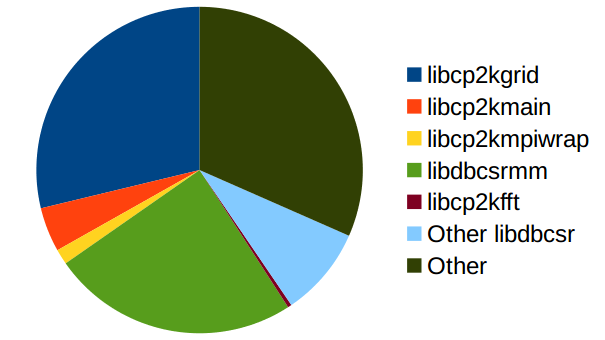
\includegraphics[width=0.45\textwidth]{images/library-performance.png}
\end{center}
\caption{Percent of Tracing by Library}
\label{fig:library-performance}
\end{figure}
